\subsection{Solução}

Para solucionar o problema da falta de comunicação entre diferentes BPMs com atividades compartilhadas, foi idealizada uma funcionalidade para integrar múltiplos BPMs com atividades que se repetem com a criação de um grande BPM agregado com múltiplas atividades iniciais.

Cada atividade inicial representa o início de um BPM, podendo existir uma ou mais atividades iniciais (como na figura~\ref{fig:bpl_completo}).
Como cada atividade inicial ainda representa uma instância daquele BPM, as informações de atividades compartilhadas entre BPMs são compartilhadas entre instâncias destes BPMs.

\begin{figure}
    \centering
    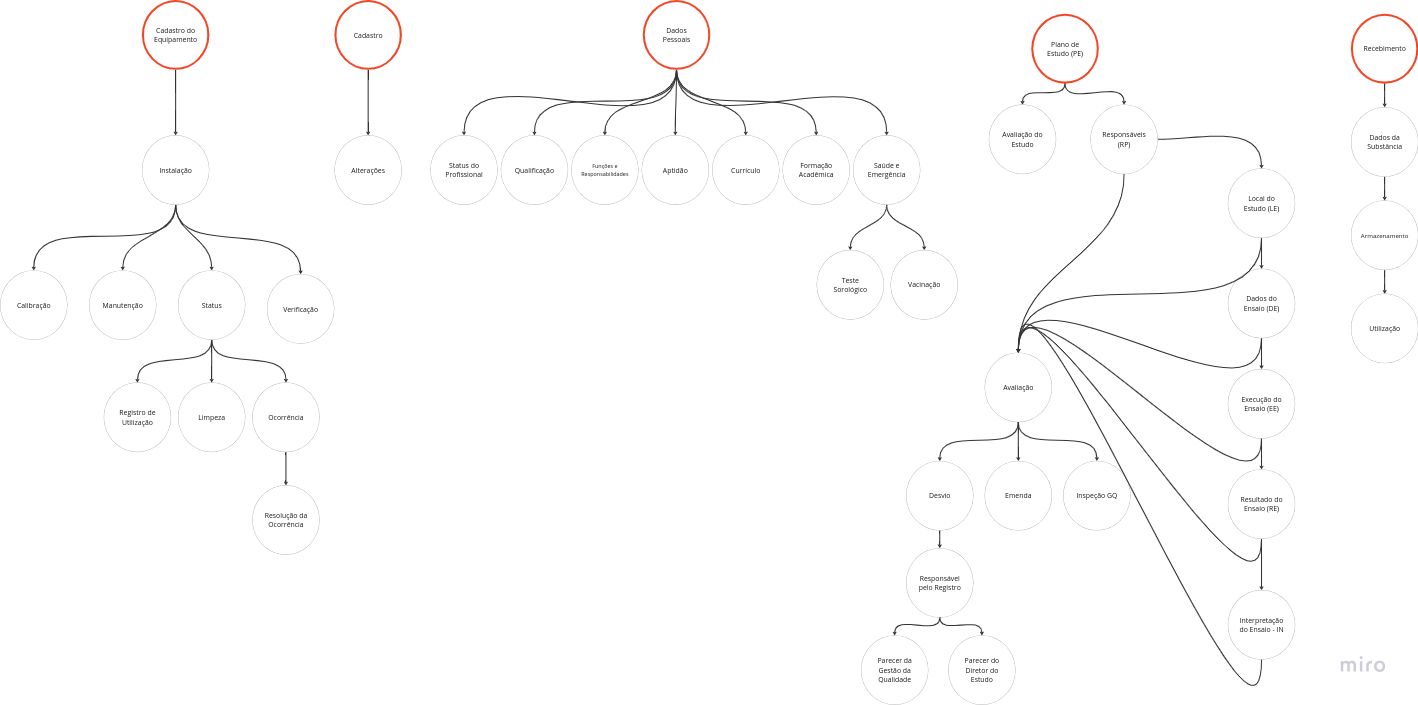
\includegraphics[width=1\textwidth]{imgs/BPL/bpl_completo.png}
    \caption{Estrutura de workflows BPL todos em um mesmo diagrama. Neste caso, cada atividade inicial (em vermelho) pode ser iniciada como uma instância no Flux.}
    \label{fig:bpl_completo}
\end{figure}

Um usuário (Ou múltiplos) criam instâncias dos BPMs compartilhados e, ao executar uma atividade compartilhada, podem escolher com quais instâncias irá compartilhar as informações contidas no mesmo.
Como exemplo, se tivermos a execução de uma atividade de pedido de exame, e existam instâncias de laboratórios de análise de amostras que compartilham da mesma atividade, o médico (usuário executando a atividade de pedido de exame) pode escolher para qual instância de laboratório essa atividade será compartilhada (como na figura~\ref{fig:arvore_medico_tecnico} citada anteriormente).

O administrador que gerencia o workflow também pode configurar permissões de atividades filhas da atividade compartilhada, podendo mostrar um fluxo de trabalho apenas para o laboratório de análise de amostras, ou seja, atividades sobre como será feito a análise estarão disponíveis apenas para os laboratórios, dando maiores possibilidades para o compartilhamento de atividades únicas.

Isso se torna útil quando se deve fazer um pedido de exame para um laboratório, o laboratório deve realizar a análise e disponibilizar os resultados para quem requisitou do exame. Neste caso, ocorre uma troca de informações assíncrona: um usuário executa uma atividade que fica disponibilizada para execução por outro usuário. Este a executa e disponibiliza o resultado para o primeiro usuário, que continua com seu fluxo de trabalho após obter os resultados.

Esta troca de informações possibilita uma maior intercomunicação entre setores da organização e aumenta a integração do LIMS onde ele está instalado, pois todas as informações, tanto de horário de requisição, quanto recebimento pelo outro usuário e execução do fluxo de trabalho compartilhado ficam armazenados no mesmo workflow.